\chapter{Firefox add-on Implementation \label{add-on}}

Firefox add-ons are a small piece of software that are used to extend and modify the installed version of Firefox by adding new features or functionality. An add-on can be used to change the theme or visual appearance of a website, add new features to the installed Firefox version, modify the user interface, add foreign language dictionaries, etc. Standard web technologies such as JavaScript, HTML and CSS are commonly used to develop a Firefox add-on ~\cite{g18}.

\section{Usability of our Firefox add-on}

We have developed a Firefox add-on to integrate TARDIS with the web browser. It scans the JavaScript from the currently open tab and alerts the user to the presence of a malicious script, hence preventing the user from any further action in the currently open tab. The central purpose of developing a Firefox add-on is to show the usability and performance evaluation of TARDIS in the browser. The add-on is entirely developed in JavaScript and hence can be integrated with other analysis tools in JavaScript.

\section{Developing a Firefox add-on}

A Firefox add-on can be developed using either of the following two methods:
\begin{enumerate}
\item WebExtensions
\item Add-on SDK
\end{enumerate}

\section{WebExtensions }

WebExtensions provide APIs for developing Firefox add-on, and is currently in the early state, but is considered to be the future of Firefox add-on development. According to ~\cite{g18}, WebExtensions will become the standard by 2017.  WebExtensions provide cross-browser compatibility, and the APIs are compatible with Google chrome and Opera's Extension API ~\cite{g18}. 

\section{Add-on SDK}

The add-on SDK method provides JavaScript APIs for Firefox add-on development and tools for creating, running, testing, and packaging them. Standard web technologies (JavaScript, CSS, HTML) are used in combination with the add-on SDK APIs.
It requires Firefox version 38 or later ~\cite{g18}. 

We have developed our Firefox add-on using the add-on SDK. At the time we started development, add-on SDK was the most stable version available.

\section{Firefox Add-on SDK installation and structure}

The add-on SDK includes the jpm for initializing, running, testing, and packaging a Firefox add-on. jpm is based on Node.js. After installation, an empty add-on is initialized by running \texttt 'jpm init' inside an empty directory. The initial directory structure of a Firefox add-on looks like the following:

\begin{figure}[htb]
\centering
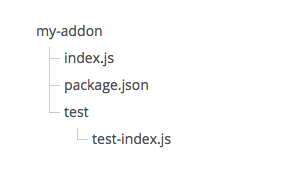
\includegraphics[width=0.5\textwidth]{image/initial_dir_struct.png}
\caption[Initial directory structure of the Firefox add-on]{Initial directory structure of the Firefox add-on ~\cite{g18}} 
\label{fig:initial_dir_struct}
\end{figure}

The figure shows the directory structure of the add-on. Here index.js is the entry point of the add-on and can be changed during the initial setup. Once the initial setup is done, Firefox add-on is developed using Add-on SDK's high-level and low-level APIs.

\section{index.js}

\begin{figure}[htb]
\centering
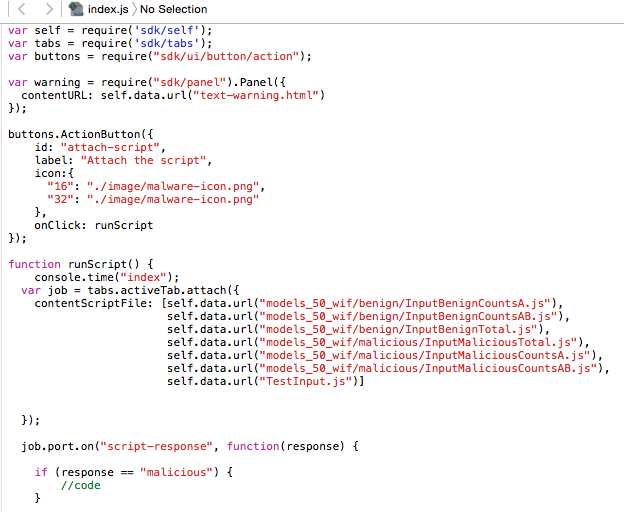
\includegraphics[width=16cm,height=25cm,keepaspectratio]{image/indexFile.png}
\caption[Index.js]{Index.js} 
\label{fig:indexFile}
\end{figure}

Index.js is the entry point of our Firefox add-on. Index.js creates and adds a button to the current version of Firefox. On the onClick event of the add-on button, function runScript gets invoked. The runScript function is responsible for invoking the SLM\_Script.js file and including the pre-build training models.

Index.js is our main add-on script. An add-on scripts can use the SDK's high-level and low-level APIs. But it does not get access to the web content directly. The add-on uses separate scripts known as content scripts to get access to the web content.  To scan the JavaScript present on the page and detect malicious content, our add-on needs to access the web page content. Some of the SDK API's, like page-mod and tabs, provide necessary functions to load content-script. Here we are loading content scripts in our main SDK script using the tabs module's attach function. The attach function is using the contentScriptFile option to load content script as a file. 

\begin{figure}[htb]
\centering
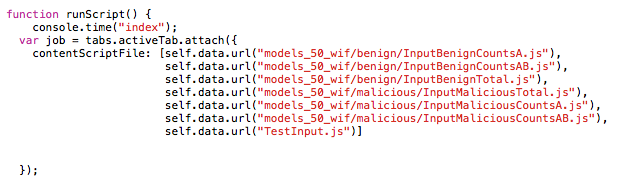
\includegraphics[width=16cm,height=20cm,keepaspectratio]{image/runScript.png}
\caption[function runScript.js]{function runscript} 
\label{fig:runScript}
\end{figure}

Tabs module is using attach () function to load the content scripts. Self.data.url(file\_name) is pointing to the file inside data directory.

\section{Content scripts}

Content scripts can access web content, but like the main add-on scripts, content-scripts can't access the SDK's APIs. Content scripts are stored as separate files under the data directory. The data directory is not created by default and needed to be added manually. We store all of our content scripts and a precompiled training model inside the data directory.  The content script can communicate back its response to the add-on script using message passing APIs.

The message communication can be done using the property port of the global object self. The sender the of message calls \texttt {port.emit} to send message and the receiver calls port.on to receive the message.

\section{Data Directory}

The data directory contains the necessary content scripts that extracts the scripts from the web page of the current open tab and classify them as either benign or malicious category. 

\begin{figure}[htb]
\centering
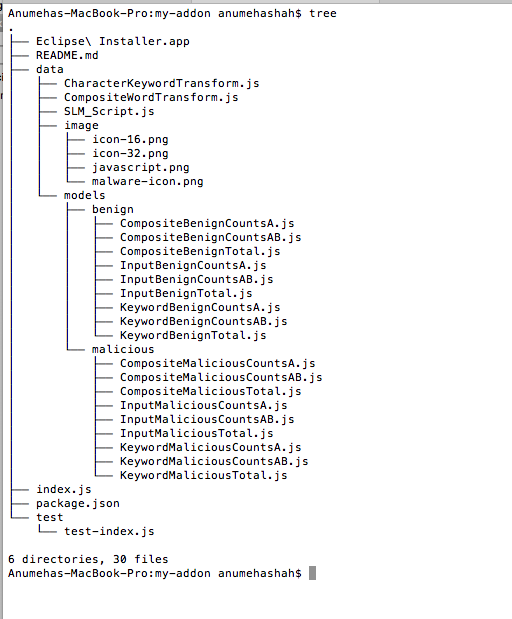
\includegraphics[width=16cm,height=30cm,keepaspectratio]{image/tree.png}
\caption[Add-on directory structure]{Add-on directory structure. Data directory contains models, image, and content scripts.} 
\label{fig:tree}
\end{figure}

\newpage

\subsection{SLM\_Script.js}

SLM\_Script.js is a content script. SLM\_Script.js extracts the JavaScript from the web page and stores it in an array and then applies algorithm to automatically generate the n-gram based benign and malicious SLM models. The script can generate the following SLM models: character level n-grams of size 3 and 4, keyword transformation n-grams of size 3 and 4, and composite word type transformation n-grams of size 3 and 4. These features are used by the precompiled benign and malicious training models to compute the overall probability of the script belonging to either of the models. The result is then passed to the add-on script index.js using \texttt{port.emit}.

\begin{figure}[htb]
\centering
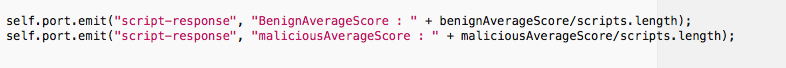
\includegraphics[width=16cm,height=20cm,keepaspectratio]{image/port-emit.png}
\caption[Example of port.emit]{Example of port.emit: SLM\_scripts.js passing the final result to the index.js} 
\label{fig:port-emit}
\end{figure}

\subsection{Models}

The Firefox add-on leverages the benefit of a pre-compiled training model for detection efficiency and better performance. The models directory inside the data directory holds all the precompiled training models required by the add-on. A script is tested on both the training model to detect the presence of malicious content. A precompiled model used within the Firefox add-on saves the overhead of sending and receiving a HTTP request to the server for the classification decision.

\section{Pre-compiled training model}

This section will present the detail discussion of the pre-compiled models we are utilizing for the add-on.

\subsection{Types of pre-compiled models}

We categorize all the training models to two categories: benign and malicious
Each of the benign and malicious categories further contains models based on character level n-grams, keyword transformation n-grams, and composite word type transformation n-grams. We are computing n-grams models of each type of size three and four. 

\newpage

\subsection{Character level n-gram model}

To compute a character level n-gram model, a file is parsed and then converted to a list of characters, then consecutive characters are joined and stored as a key-value pair in JSON format. A key is the n-gram/feature and the value is the frequency of occurrence in the script. This type of model presents the content of the document more than the structure.

\begin{figure}[htb]
\centering
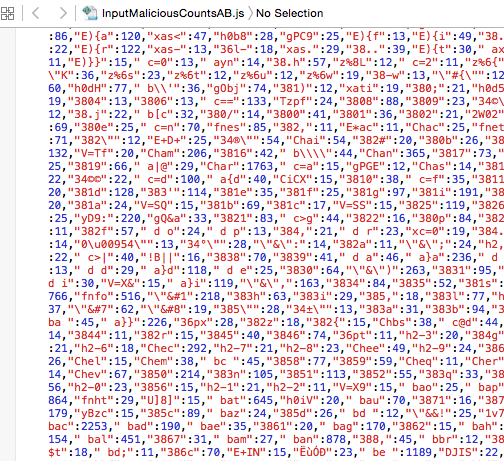
\includegraphics[width=16cm,height=20cm,keepaspectratio]{image/character.png}
\caption[A snapshot of a pre-compiled malicious character level n-grams model]{A snapshot of a pre-compiled malicious character level n-grams model of size 4. Every key is four characters long} 
\label{fig:character}
\end{figure}

\subsection{Keyword transformation}

Keyword transformation parse the script and converted it into a list of characters, then join the consecutive characters to form n-grams. Keyword transformation is similar to character level n-grams, but in keyword transformation, reserved keywords are stored with the whole word as a single token. Keyword transformation preserves both the content and the semantics of a script.

\begin{figure}[htb]
\centering
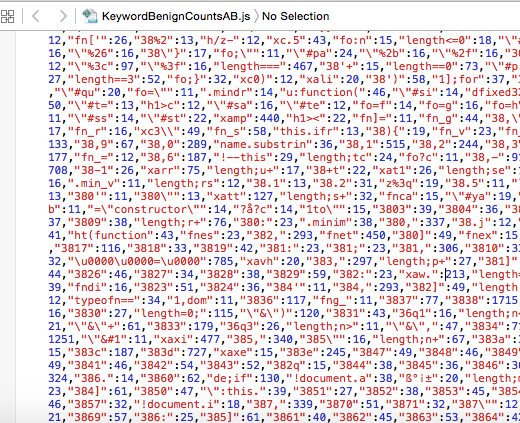
\includegraphics[width=16cm,height=20cm,keepaspectratio]{image/keyword.png}
\caption[a snapshot of a keyword transformation n-grams model]{a snapshot of a keyword transformation n-grams model. Reserved keyword such as length, constructor, and min appear as the whole word combined with the consecutive characters that are not part of the reserved keyword} 
\label{fig:keyword}
\end{figure}

\subsection{Composite word type transformation}
Composite word type transformation converts the sequence of characters into distinct classes. Here the following classes are used to represent characters: DIGIT, HEX, WHITESPACE, PUNCTUATION, and PERCENT. Characters other than these categories are joined and represent a single token. These classes and tokens are combined to form composite word type n-grams of size there and four. As discussed in the section \ref{n-grams}, composite word type transformation reduces entropy in an obfuscated malicious program.

\begin{figure}[htb]
\centering
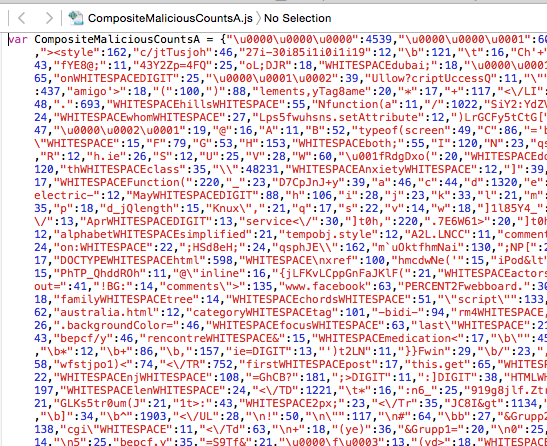
\includegraphics[width=16cm,height=15cm,keepaspectratio]{image/composite.png}
\caption[A snapshot of the malicious n-grams composite word type transformation model ]{A snapshot of the malicious n-grams composite word type transformation model} 
\label{fig:composite}
\end{figure}

\subsection{Precompiled training models computation}

The models are computed using the TARDIS source program in Java. TARDIS is written in java. The source code first computes the training model and uses the training model to test the JavaScript for malicious or benign categorization. We leverage this functionality and store the model generated by TARDIS persistently in JSON format. The primary reason behind storing a model in JSON format is that a JSON is light weight and portable. Storing a model in JSON with the add-on would not take much space in the browser and it can also provide a quick look up of key-value pair.

\begin{figure}[htb]
\centering
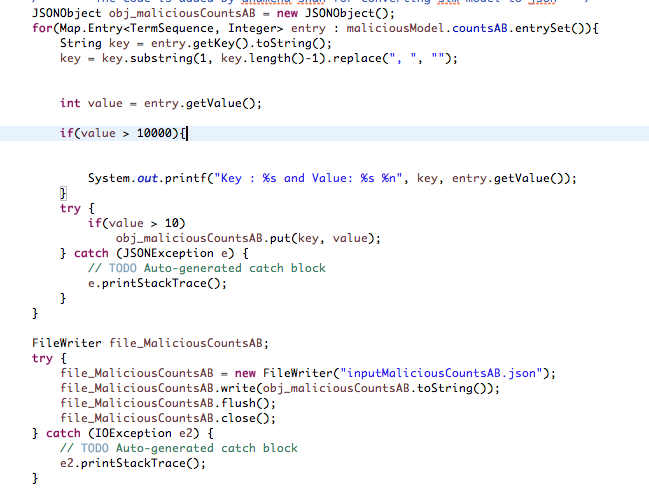
\includegraphics[width=16cm,height=15cm,keepaspectratio]{image/model-computation.png}
\caption[Java code added for model computation ]{Java code added for model computation} 
\label{fig:model-computation}
\end{figure}

\subsection{Problems faced during pre-compiled model generation and solution implementation}

The model generation for large no of files is computationally expensive process.
For efficient processing and time reduction for model generation, we implemented a multithreading solution to the existing TARDIS model generation algorithm. The multithreading reduces execution time by roughly two-third. 

\begin{figure}[htb]
\centering
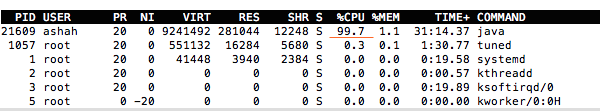
\includegraphics[width=16cm,height=15cm,keepaspectratio]{image/cpu-per-1.png}
\caption[CPU utilization before multithreading implementation]{output of top command before multithreading implementation
shows \% CPU utilization as 99.7\%} 
\label{fig:cpu-per-1}
\end{figure}

\begin{figure}[htb]
\centering
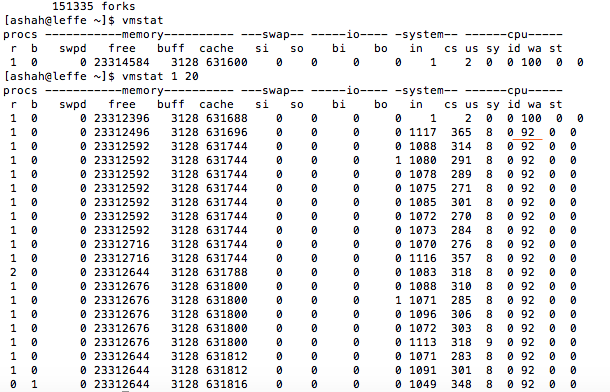
\includegraphics[width=16cm,height=15cm,keepaspectratio]{image/cpu-wa-1.png}
\caption[CPU idle time before multithreading implementation]{CPU idle time before multithreading implementation = 92} 
\label{fig:cpu-wa-1}
\end{figure}

CPU utilization percentage and idle time after multithreading implementation.

\begin{figure}[htb]
\centering
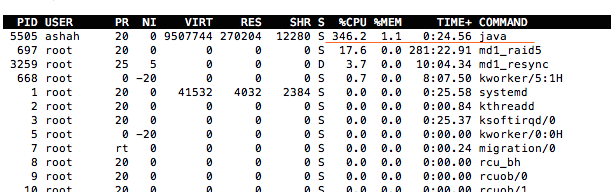
\includegraphics[width=16cm,height=25cm,keepaspectratio]{image/cpu-per-2.png}
\caption[CPU utilization after multithreading implementation]{output of top command after multithreading implementation
shows \% CPU utilization as 346.2\%} 
\label{fig:cpu-per-2}
\end{figure}

\bigskip

\begin{figure}[htb]
\centering
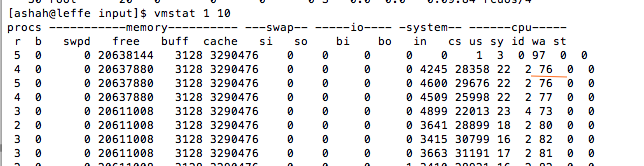
\includegraphics[width=16cm,height=25cm,keepaspectratio]{image/cpu-wa-2.png}
\caption[CPU idle time after multithreading implementation]{CPU idle time after multithreading implementation = 76} 
\label{fig:cpu-wa-2}
\end{figure}

\newpage



\section{Result Computation}

The add-on computes the overall probability of a script over the benign and malicious model. For each n-gram the mode looks for the frequency value in n-grams of size 3 model and n-grams of size 4 JSON model. The model then computes the overall probability of the script for both the benign and malicious models using the formula

\[Probability = probability + math.log(pAB/pA)\]


pAB = (frequency of n-grams of size 4)/ (total no of words)

pA = (frequency of the n-grams of size 3)/(total no of words)




